\documentclass[11pt,letterpaper]{article}

\usepackage[utf8x]{inputenc}
\usepackage{ucs}
\usepackage[spanish]{babel}
\usepackage{amsmath}
\usepackage{amsfonts}
\usepackage{amssymb}
\usepackage{graphicx} % Para importar imagenes
\graphicspath{{../img/}} % Ruta de imagenes

\author{J. Mauricio Mejía Castro}
\title{Probabilidad y Estadística para Análisis de Datos - Solución al Taller No. 2}

\begin{document}

\maketitle

\section{Resumen de Información en Tablas}
El Cuadro \ref{tab:table-01} compila el cálculo de la media, la mediana y el coeficiente de variación para las ocho variables numéricas del conjunto de datos. Además, estos resultados se encuentran agrupados por la variable {\tt class}. \\
De acuerdo con el Cuadro \ref{tab:table-01} pueden observarse diferencias significativas de las variables con respecto a la clase. Por ejemplo, es claro que para aquellas mujeres con resultado negativo para diabetes, la media de las variables es menor. Un fenómento similar ocurre con las medianas. No obstante, se observa también que el coeficiente de variación es mayor para las mujeres con resultado negativo para diabetes: existe mayor incertidumbre en los datos de esta clase.

\begin{table}[t]
\centering
\begin{tabular}{|c|c|c|} \hline
{\sc class} & {\sc Negativo para diabetes} & {\sc Positivo para diabetes}\\ \hline
preg\_media & 3.298 & 4.86567164179105\\ 
plas\_media & 109.98 & 141.257462686567\\ 
pres\_media & 68.184 & 70.8246268656716\\ 
skin\_media & 19.664 & 22.1641791044776\\ 
test\_media & 68.792 & 100.335820895522\\ 
mass\_media & 30.3042 & 35.1425373134328\\ 
pedi\_media & 0.429734 & 0.5505\\ 
age\_media & 31.19 & 37.0671641791045\\ \hline
preg\_mediana & 2 & 4\\ 
plas\_mediana & 107 & 140\\ 
pres\_mediana & 70 & 74\\ 
skin\_mediana & 21 & 27\\ 
test\_mediana & 39 & 0\\ 
mass\_mediana & 30.05 & 34.25\\ 
pedi\_mediana & 0.336 & 0.449\\ 
age\_mediana & 27 & 36\\  \hline
preg\_coevar & 91.4852814621555 & 76.8904956904246\\ 
plas\_coevar & 23.7690486955388 & 22.6109272038089\\ 
pres\_coevar & 26.4916628729699 & 30.3451110181861\\ 
skin\_coevar & 75.7218628648506 & 79.7670480694412\\ 
test\_coevar & 143.716259582972 & 138.224936511905\\ 
mass\_coevar & 25.3755420425225 & 20.6671680464296\\ 
pedi\_coevar & 69.5977754511886 & 67.6393248963871\\ 
age\_coevar & 37.4083193062878 & 29.5902152087236\\  \hline
\end{tabular}
\caption{Cálculo de estadísticas descriptivas agrupado por clase para todas las variables del conjunto de datos.}
\label{tab:table-01}
\end{table}

\section{Resumen de Información en Gráficas}

La Figura \ref{fig:figure-01} contiene un diagrama de dispersión entre el índice de masa corporal y el espesor del pliegue cutáneo ubicado sobre el músculo triceps. La gráfica refleja cierta linealidad difusa entre las dos variables. Cabe destacar también el elevado número de valores inexistentes para la variable {\tt skin}.


\begin{figure}[h]
\centering
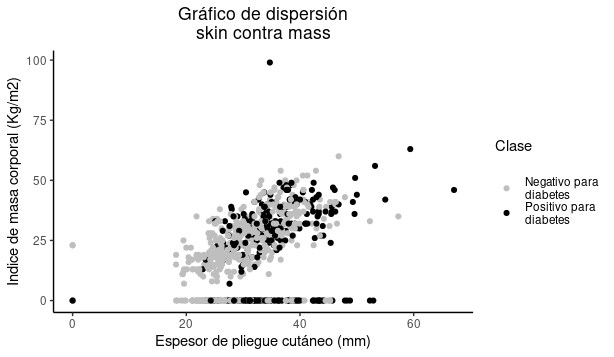
\includegraphics[scale=0.7]{scatter0.png}
\caption{Gráfica de dispersión para las variables {\tt mass} y {\tt skin}.}
\label{fig:figure-01}
\end{figure}

Además del grafico de dispersión, se construyeron también los diagrama de caja de la Figura \ref{fig:figure-02}, debido a su capacidad para identificar valores atípicos. Allí se podrá apreciar la distribución de los datos, teniendo en cuanta la clase. Es posible ver como el espesor del pliegue cutáneo tiende a ser menor en las mujeres con resultado positivo para diabetes y como estas mismas mujeres tienden  a registrar mayores IMC.

\begin{figure}
\centering
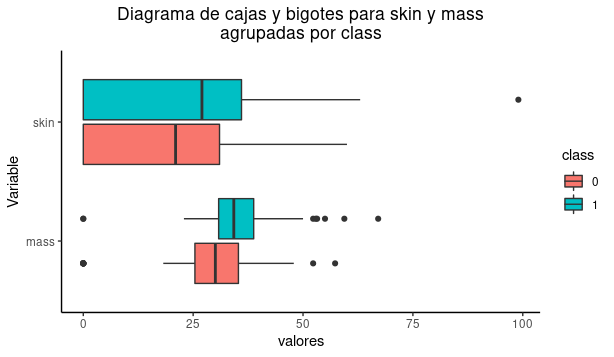
\includegraphics[scale=0.6]{boxplot0.png}
\caption{Diagrama de cajas y bigotes para las variables {\tt mass} y {\tt skin}.}
\label{fig:figure-01} 
\end{figure}




\section{Exploración de correlaciones}
Para esta sección resulta valioso observar lás gráficas de densidad de las variables {\tt mass} y {\tt skin} que se encuentran en la Figura \ref{fig:figure-03}.

A partir de estás gráficas es claro que las variables no tienden a distribuirse normalmente. Por consiguiente, no es recomendable utilizar el coeficiente de Pearson para determinar la correclación entre ellas. Es por esta razón que se prefiere el coeficiente de Kendall.

Dado que se desconoce la razón de aquellos valores, que marcan cero para {\tt mass} y {\tt skin}, se opta por seguir incluyendolos en el análisis. En este punto, solo la asesoría de una opinion experta en el conjunto de datos podría disuadir esta decisión.

\begin{figure}
\centering
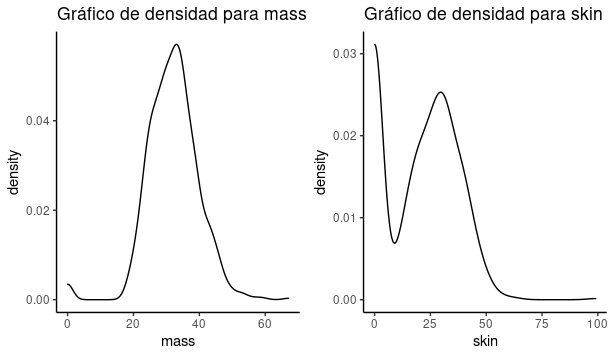
\includegraphics[scale=0.6]{density_array.png}
\caption{Distribuciones de las variables {\tt mass} y {\tt skin}.}
\label{fig:figure-03} 
\end{figure}


Al ejecutar el test de correlación en R, obtenemos el siguiente resultado:

\begin{verbatim}
> cor.test(diabetis$mass, diabetis$skin, method = "kendall")
\end{verbatim}

\begin{verbatim}
	Kendall's rank correlation tau

data:  data.diabetis$mass and data.diabetis$skin
z = 13.18, p-value < 2.2e-16
alternative hypothesis: true tau is not equal to 0
sample estimates:
      tau 
0.3315319 
\end{verbatim}

Este test arroja un {\tt p-value} muy bajo. No obstante, no secuentan en este punto con herramientas más formalesque permitan decidir sieste valor es significativamente diferente de cero. Por consiguiente, aun no puede concluirse nada sobre la correlación entre estas variables.

\end{document}